\begin{frame}{What is \emph{Machine Learning}? -- A brief introduction}
\begin{center}
\begin{tikzpicture}
\clip (-4.25, 1.125) rectangle (4.25,-4.5);

\def\imgsize{2}

\draw (0,0) coordinate (center);

\draw (center) node (icon) {
\includegraphics[width=\imgsize cm]{\PhDthesisdir/plots_and_images/misc_for_slides/machine.png}} ;
\draw [thick, rounded corners = 5pt] (center)+(-\imgsize/2,-\imgsize/2) rectangle +(\imgsize/2,\imgsize/2);
\draw (center)+(0,-\imgsize/2) node [below] {\scriptsize Classical};

\draw (icon.east) [thick, -latex] --+ (\imgsize/1.5,0) node [right] {Output};

\draw (icon.west)+(0,\imgsize/3) [thick, latex-] --+ (-\imgsize/1.5,\imgsize/3) node [left] {Input};
\draw (icon.west)+(0,-\imgsize/3) [thick, latex-] --+ (-\imgsize/1.5,-\imgsize/3) node (P1) [left] {Program};

%\draw (0,{-1.5*\imgsize}) coordinate (center);
%
%\draw (center) node (icon) {
\includegraphics[width=\imgsize cm]{\PhDthesisdir/plots_and_images/misc_for_slides/machine.png}} ;
%\draw [thick, rounded corners = 5pt] (center)+(-\imgsize/2,-\imgsize/2) rectangle +(\imgsize/2,\imgsize/2);
%\draw (center)+(0,-\imgsize/2) node [below] {\scriptsize Machine Learning};
%
%\draw (icon.east) [thick, -latex] --+ (\imgsize/1.5,0) node (P2) [right] {Program};
%
%\draw (icon.west)+(0,\imgsize/3) [thick, latex-] --+ (-\imgsize/1.5,\imgsize/3) node [left] {Input};
%\draw (icon.west)+(0,-\imgsize/3) [thick, latex-] --+ (-\imgsize/1.5,-\imgsize/3) node [left] {Output};
%
%\draw [thick, -latex] (P2) to [in=-90, in looseness = 0.65, out=90, out looseness = 0.65] (P1);
\end{tikzpicture}
\end{center}
\end{frame}

\addtocounter{framenumber}{-1}
\begin{frame}{What is \emph{Machine Learning}? -- A brief introduction}
\begin{center}
\begin{tikzpicture}
\clip (-4.25, 1.125) rectangle (4.25,-4.5);

\def\imgsize{2}

\draw (0,0) coordinate (center);

\draw (center) node (icon) {
\includegraphics[width=\imgsize cm]{\PhDthesisdir/plots_and_images/misc_for_slides/machine.png}} ;
\draw [thick, rounded corners = 5pt] (center)+(-\imgsize/2,-\imgsize/2) rectangle +(\imgsize/2,\imgsize/2);
\draw (center)+(0,-\imgsize/2) node [below] {\scriptsize Classical};

\draw (icon.east) [thick, -latex] --+ (\imgsize/1.5,0) node [right] {Output};

\draw (icon.west)+(0,\imgsize/3) [thick, latex-] --+ (-\imgsize/1.5,\imgsize/3) node [left] {Input};
\draw (icon.west)+(0,-\imgsize/3) [thick, latex-] --+ (-\imgsize/1.5,-\imgsize/3) node (P1) [left] {Program};

\draw (0,{-1.5*\imgsize}) coordinate (center);

\draw (center) node (icon) {
\includegraphics[width=\imgsize cm]{\PhDthesisdir/plots_and_images/misc_for_slides/machine.png}} ;
\draw [thick, rounded corners = 5pt] (center)+(-\imgsize/2,-\imgsize/2) rectangle +(\imgsize/2,\imgsize/2);
\draw (center)+(0,-\imgsize/2) node [below] {\scriptsize Machine Learning};

\draw (icon.east) [thick, -latex] --+ (\imgsize/1.5,0) node (P2) [right] {Program};

\draw (icon.west)+(0,\imgsize/3) [thick, latex-] --+ (-\imgsize/1.5,\imgsize/3) node [left] {Input};
\draw (icon.west)+(0,-\imgsize/3) [thick, latex-] --+ (-\imgsize/1.5,-\imgsize/3) node [left] {Output};
%
%\draw [thick, -latex] (P2) to [in=-90, in looseness = 0.65, out=90, out looseness = 0.65] (P1);
\end{tikzpicture}
\end{center}
\end{frame}

\addtocounter{framenumber}{-1}
\begin{frame}{What is \emph{Machine Learning}? -- A brief introduction}
\begin{center}
\begin{tikzpicture}
\clip (-4.25, 1.125) rectangle (4.25,-4.5);

\def\imgsize{2}

\draw (0,0) coordinate (center);

\draw (center) node (icon) {
\includegraphics[width=\imgsize cm]{\PhDthesisdir/plots_and_images/misc_for_slides/machine.png}} ;
\draw [thick, rounded corners = 5pt] (center)+(-\imgsize/2,-\imgsize/2) rectangle +(\imgsize/2,\imgsize/2);
\draw (center)+(0,-\imgsize/2) node [below] {\scriptsize Classical};

\draw (icon.east) [thick, -latex] --+ (\imgsize/1.5,0) node [right] {Output};

\draw (icon.west)+(0,\imgsize/3) [thick, latex-] --+ (-\imgsize/1.5,\imgsize/3) node [left] {Input};
\draw (icon.west)+(0,-\imgsize/3) [thick, latex-] --+ (-\imgsize/1.5,-\imgsize/3) node (P1) [left] {Program};

\draw (0,{-1.5*\imgsize}) coordinate (center);

\draw (center) node (icon) {
\includegraphics[width=\imgsize cm]{\PhDthesisdir/plots_and_images/misc_for_slides/machine.png}} ;
\draw [thick, rounded corners = 5pt] (center)+(-\imgsize/2,-\imgsize/2) rectangle +(\imgsize/2,\imgsize/2);
\draw (center)+(0,-\imgsize/2) node [below] {\scriptsize Machine Learning};

\draw (icon.east) [thick, -latex] --+ (\imgsize/1.5,0) node (P2) [right] {Program};

\draw (icon.west)+(0,\imgsize/3) [thick, latex-] --+ (-\imgsize/1.5,\imgsize/3) node [left] {Input};
\draw (icon.west)+(0,-\imgsize/3) [thick, latex-] --+ (-\imgsize/1.5,-\imgsize/3) node [left] {Output};

\draw [thick, -latex] (P2) to [in=-90, in looseness = 0.65, out=90, out looseness = 0.65] (P1);
\end{tikzpicture}
\end{center}
\end{frame}

\begin{frame}{What is \emph{Machine Learning}? -- A brief introduction}

\begin{center}
\textbf{Aim}: find a function (program) mapping features (input) to a target (output)
\end{center}

\pause
\begin{minipage}[t]{.45\textwidth}
\manip Categorical target $\Rightarrow$ Classification\\
\qquad\eg\ cat or dog on the image
\begin{center}
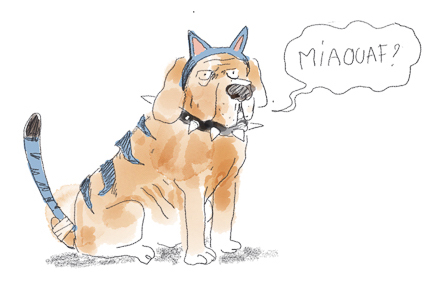
\includegraphics[width=.8\linewidth]{\PhDthesisdir/plots_and_images/misc_for_slides/datafrog_chien_chat.jpeg}
\end{center}
\end{minipage}
\hfill\pause
\begin{minipage}[t]{.45\textwidth}
\manip Continuous target $\Rightarrow$ Regression\\
\qquad\eg\ discriminating variable!

Linear case:
\begin{center}
\includegraphics[width=.8\linewidth]{\PhDthesisdir/plots_and_images/misc_for_slides/linear_regression_example/fig-linear_regression_example-wrapper.tex}
\end{center}

What if the target is not linear wrt. input?
\end{minipage}

\end{frame}